\documentclass{ceri}
\title{Preliminary Design Alternatives Report}
\usepackage[final]{pdfpages}
\usepackage[driver=pdftex]{geometry}
\addbibresource{bibliographie.bib}
\usepackage{longtable}
\usepackage[colorlinks=true]{hyperref}
\tolerance=1
\emergencystretch=\maxdimen
\hyphenpenalty=10000
\hbadness=10000
\widowpenalty10000
\clubpenalty10000
\newcommand{\myparagraph}[1]{\paragraph{#1}\mbox{}\\}
\usepackage{etoolbox,refcount}
\usepackage{multicol}
\usepackage{graphicx}
\usepackage{booktabs}
\usepackage{lscape}
\usepackage[table,xcdraw]{xcolor}
\newcounter{countitems}
\newcounter{nextitemizecount}
\newcommand{\setupcountitems}{%
  \stepcounter{nextitemizecount}%
  \setcounter{countitems}{0}%
  \preto\item{\stepcounter{countitems}}%
}
\makeatletter
\newcommand{\computecountitems}{%
  \edef\@currentlabel{\number\c@countitems}%
  \label{countitems@\number\numexpr\value{nextitemizecount}-1\relax}%
}
\newcommand{\nextitemizecount}{%
  \getrefnumber{countitems@\number\c@nextitemizecount}%
}
\newcommand{\previtemizecount}{%
  \getrefnumber{countitems@\number\numexpr\value{nextitemizecount}-1\relax}%
}
\makeatother    
\newenvironment{AutoMultiColItemize}{%
\ifnumcomp{\nextitemizecount}{>}{3}{\begin{multicols}{2}}{}%
\setupcountitems\begin{itemize}}%
{\end{itemize}%
\unskip\computecountitems\ifnumcomp{\previtemizecount}{>}{3}{\end{multicols}}{}}
\newcommand{\namesigdate}[2][5cm]{%
  \begin{tabular}{@{}p{#1}@{}}
    #2 \\[2\normalbaselineskip] \hrule \\[0pt]
    {\small \textit{Signature}} \\[2\normalbaselineskip] \hrule \\[0pt]
    {\small \textit{Printed Name}}\\[2\normalbaselineskip] \hrule \\[0pt]
    {\small \textit{Title}}\\[2\normalbaselineskip] \hrule \\[0pt]
    {\small \textit{Date}}
  \end{tabular}
}

\begin{document} 
\maketitle
\sloppy     

\section{Cover Letter}
\setlength{\parindent}{0pt}
February 4, 2019
\newline

\newpage
\setlength{\parindent}{8pt}
\pagenumbering{arabic}
\section{Executive Summary}
Text Here: Insert Text Here
\section{Project Understanding}

\subsection{Purpose}
This report was prepared for Keiwit Power by TechnologyBin and submitted on February 18, 2019. The purpose of the report is to outline conceptional design alternatives that will be considered for Keiwit Power’s Combined Cycle power generating station project in the Memphis, Tennessee area. Our engineers have provided several alternative design options for six aspects of the project design. Each design option has been evaluated based on criteria relative to the respective design aspect.

\newpage

\subsection{Project Summary}
TechnologyBin will design a combined cycle power generating station for Keiwit Power. The Combined Cycle (CC) electricity generating plant will consist of two combustion turbine-generators, two heat recovery steam generators with supplemental firing capability, and one steam turbine-generator. The key design aspects of the project that TechnologyBin will be responsible for are as follows:

\begin{itemize}
\item 	A multifunctional administrative building 	
\begin{itemize}
\item Structural and foundation design
\item 	Design of mechanical systems such as heating, ventilation, and air-conditioning systems and lighting system
\end{itemize}
\item 	Site design
\begin{itemize}
\item 	Site grading and drainage
\item 	Transportation
\item 	Landscaping
\end{itemize}
\item 	Water supply system
\begin{itemize}
\item Greywater supply
\item 	Potable water supply from local water district
\item 	Service/fire water storage
\item 	Demineralized water production system
\end{itemize}
\item 	Chemical Storage	
\begin{itemize}
\item Two permanent liquid nitrogen storage tanks
\item 	Two permanent CO2 storage tanks
\item 	Two welded steel aqueous ammonia storage tanks
\item 	Chemical feed building to provide storage for water treatment chemicals
\item 	A dedicated outdoor stall including a manifold and connections for tractor-trailer tankers containing hydrogen
\end{itemize}
\item 	Plant water discharge system
\begin{itemize}
\item 	Industrial wastewater system including two wastewater blowdown tanks, a metered discharge pipe system, and a 12,000-gallon combustion turbine wash-water catch tank
\item  	Sanitary sewer system routed to the local sanitary sewer
\newline
\end{itemize}
\end{itemize}
\newpage
The administrative building will provide facilities for operational, maintenance, and administrative support staff totaling about 30 regular employees. The roughly 20,000 square foot building will be comprised of three separate areas: an office area, a warehouse area, and a control/engineering area. A two-hour rated firewall will separate the office area from the control/engineering area as well as the office area from the warehouse area. One doorway per firewall will allow access to adjoining areas. Each area will have an entry/exit airlock doorway to the rest of the plant.\\
\newline

A transportation network of roads will allow workers access to the plant as well as provide an adequate surface to operate equipment such as forklifts between buildings. Paved surfaces on the site will include gutters with oil and chemical traps in case of spill being introduced into the site drainage system.\\
\newline

The water supply system will include a greywater treatment system capable of producing service water that will be stored in the service water/fire water storage tanks. The storage tanks will maintain a service water reserve of at least 260,000 gallons for fire suppression while supplying the water demineralization system. The demineralized water will be used in the production of steam to run the steam turbine generator.\\
\newline

Waste water expelled from the plant will be managed base on the potential contaminants. A separate sanitary sew system will be used to manage waste water suitable for the county sanitary sewer system.


\newpage
\subsection{Site Location}
The proposed project site will be located roughly five miles southwest of downtown Memphis, Tennessee inside the Frank C. Pidgeon Industrial Park. \textbf{Figure \ref{fig:Location}} depicts the proposed project site boundaries and location. 
\begin{figure}[H]
    \centering
    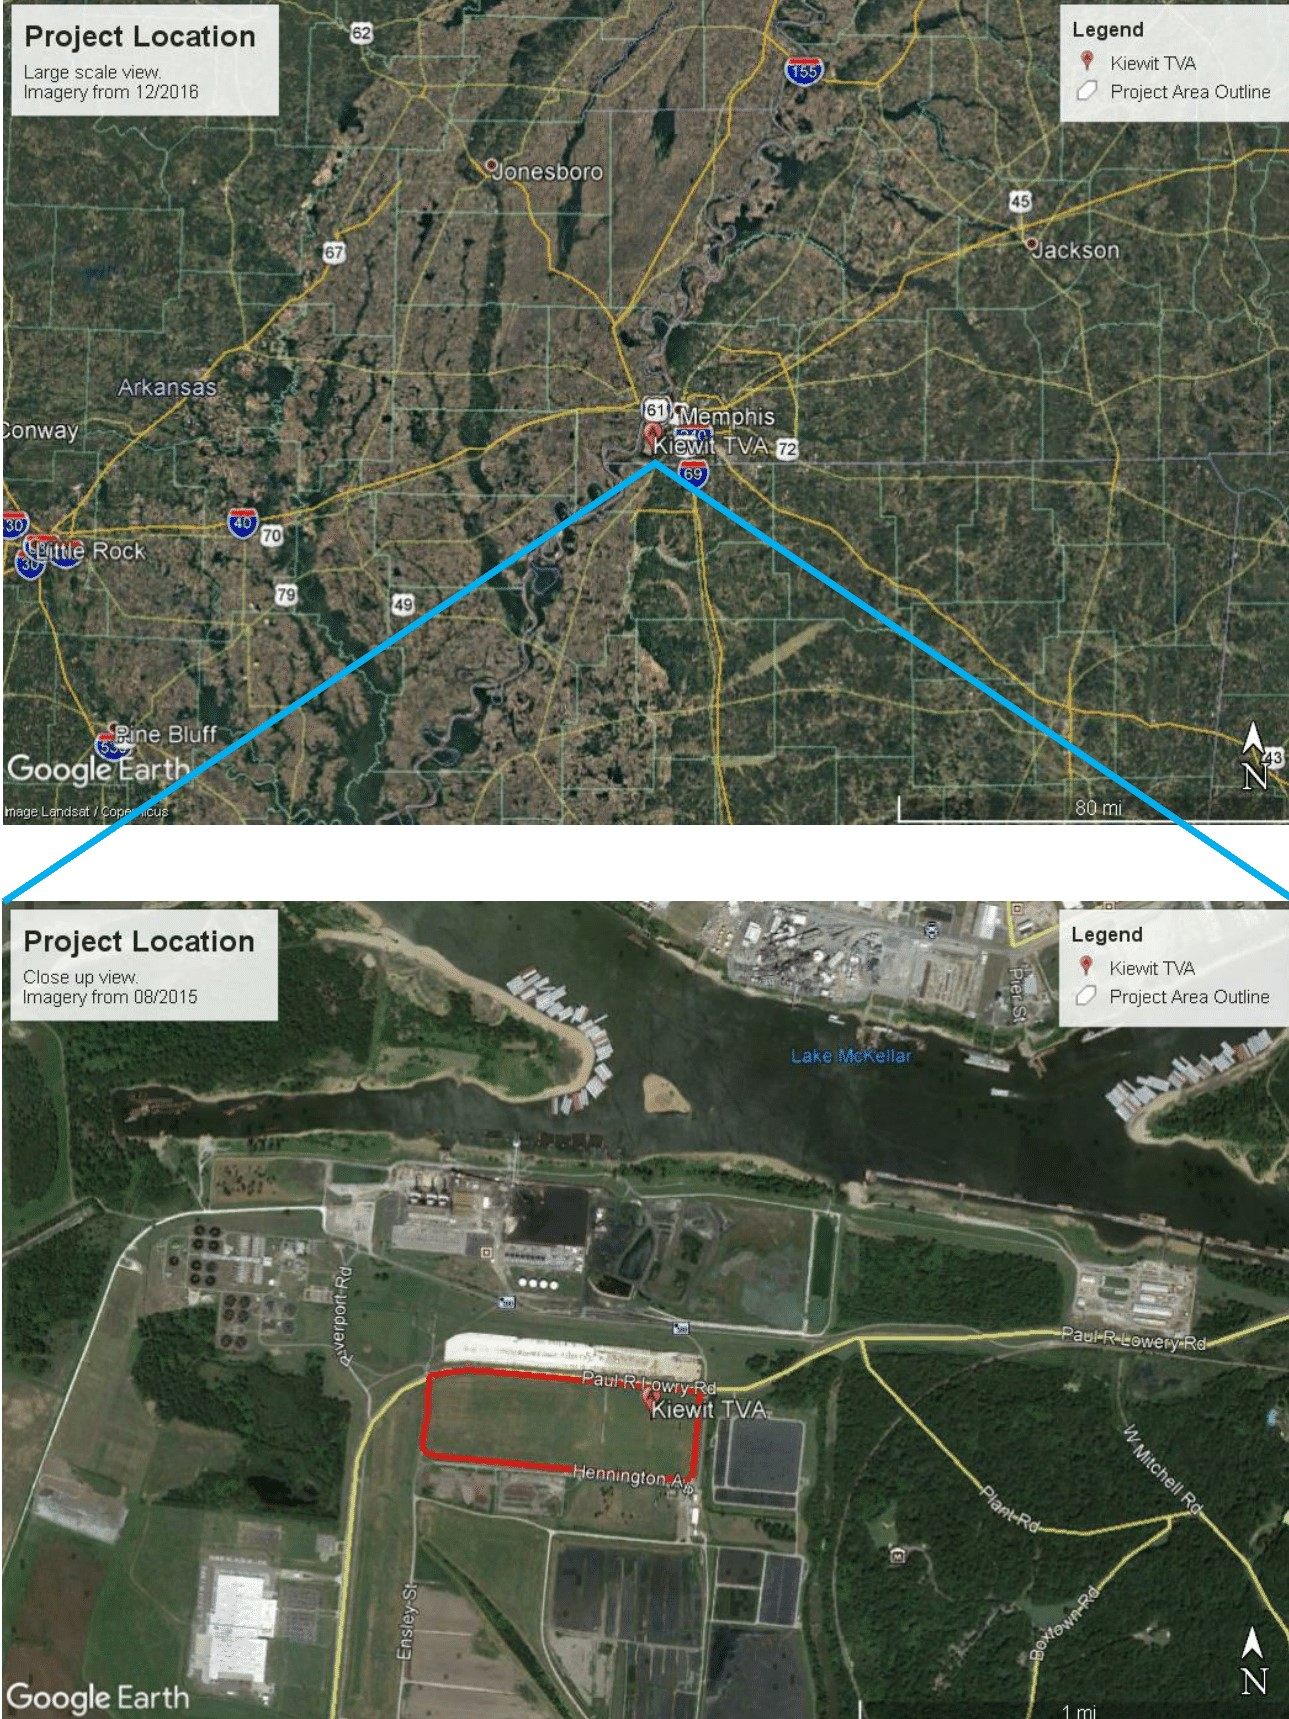
\includegraphics[width=.85\textwidth]{images/Location.png}
    \caption{Aerial View of Project Site}
    \label{fig:Location}
\end{figure}
\section{Engineers scope of Work}


\subsection{Civil Engineering}
TechnologyBin’s civil engineering team includes engineers specializing in structural design, geotechnical/foundation design, and site development.\\
\newline

Our structural engineers will develop an economical design while cooperating with our geotechnical engineers in development of a foundation design. The structural and foundation designs of the plant will be developed in accordance with the state’s latest edition of the Uniform Statewide Building Code, ASTM, AISC, ACI, IBC 2009, and ASCE 7-10.\\
\newline

Our geotechnical engineers will conduct site analysis and review geotechnical reports such as boring log results, rock core analysis, lab reports from designated testing, and other geologic data to aid in the development of the foundation design. This includes proper compaction testing to reduce pumping infill and excavation areas.\\
\newline
The site development team will develop the site grading plan based on foundation design requirements, site topography, and soil classification/characteristics. The team will also maintain collaboration with the structural and foundation design teams to designate adequate design parameters.\\
\newline

The team will also develop stormwater runoff and drainage design and transportation plans. The stormwater runoff and drainage design will reduce erosion by directing the runoff to designated locations on the property. Transportation will include roadway design for ease and safe access throughout the development of the site, parking lot design, and sidewalk design. During the designing phase, the site development team will work with the Tennessee’s Department of Transportation to approve access to the proposed facility. Appropriate design requirements and regulations will be met during this process. This process will also include utility layout and design through collaboration with the utility manager.
\newpage
All phases of site development will follow the designated design procedures and specifications made by the client as well as design codes within the state’s Uniform Statewide Building Code and any codes required by Shelby County. 

\subsection{Architectural Engineering}
Our architectural engineers will be responsible for the design of the site layout as well as the buildings on the site and their respective HVAC and lighting systems.\\
\newline

The buildings included in the project design will provide a functional and efficient workspace for the employees of the power plant. They will be designed to serve a variety of purposes and oriented within the site layout design in manner to provide ease of access. The administrative building and associated facilities will be designed in accordance with Americans with Disabilities Act (ADA). When possible, materials will be chosen to benefit the local community and to minimize environmental impact on the surrounding area.\\
\newline

The lighting on both the interior and exterior of the buildings will provide a safe working environment for employees while adding aesthetic appeal. Exterior plant lighting will be designed to reduce outward glare. Natural light will be utilized to decrease the demand for electrical lighting and to create more productive workspaces. Energy-efficient light sources, such as LED lighting, will be used to enhance the lifetime of the building and to reduce energy waste.\\
\newline
Systems that control the environment within the buildings will be designed to keep occupants comfortable and healthy while inside the facilities. Our team will design heating, ventilation, and air-conditioning (HVAC) systems in accordance with American Society of Heating, Refrigeration, and Air-Conditions Engineers (ASHRAE) standards. This style of design will provide a sustainable space as well as protect the health of employees and guests.
\newpage
\subsection{Environmental Engineering}
Our environmental engineers will be responsible for reduction of the environmental impact of the project through efficient management of air emissions as well as stormwater runoff control. They will also design a greywater treatment system and a plant waste water discharge system.\\
\newline

The quality of air directly impacts the employees at the facility and the surrounding community. It is vital that the environmental team adheres to regulations and standards that apply to air quality control.\\
\newline

Air abatement controls will include a low NOx burner, a selective catalyst reduction system (SCR), and a carbon monoxide catalyst. The environmental engineering team will investigate the impact of atmospheric emissions of NOx by the plant under current abatement control methods. The EPA’s atmospheric dispersion modeling system (AERMOD) and diagnostic Stationary Wind Field and Turbulence model (SWIFT) will be utilized to simulate emissions under worst-case meteorological conditions and three 10-day periods representative of typical atmospheric.\\
\newline

Stormwater management will be a major concern on this project due to the site’s proximity to the Mississippi River. The environmental engineering team will perform a complete analysis of the site and prepare a plan to prevent flood damage to the buildings and systems. The team will work closely with the site development team in the design of the layout of the water drainage system. This drainage will serve to protect the surrounding environment from excessive erosion by effectively dispersing runoff from developed surfaces. \\
\newline

The plant water discharge system will include an industrial wastewater system and a sanitary sewer system. Two wastewater blowdown tanks will be utilized for collection of waste water from cooling tower blowdown. The discharge pipe from the blowdown tanks will be equipped with a metering system to measure discharge flow. A 12,000-gallon water wash tank will be utilized in collection of waste water from combustion turbine wash cycles. Areas around equipment with potential for oil spills will be paved and curbed to allow runoff to flow to an oil/water separator before discharge to the cooling tower basin. Chemical handling areas will be paved and curbed to allow water runoff to flow to a chemical waste slump before discharge to the cooling tower basin. Sanitary wastewater from the plant will be routed to the local sanitary sewer. 

\subsection{Construction}
Our construction manage team will provide project cost estimation and scheduling services.

Cost estimation will encompass all stages involved in the design and construction process for the proposed site. Estimates will be handled by professionals at TechnologyBin to develop a suitable budget for the project to aid management of costs throughout the design and the construction phases. This includes labor, materials used during construction, utilities, foundations, structural components, and other equipment or materials used in the project.\\
\newline

The construction management team will also provide a detailed schedule to outline the tasks and subtasks to be completed throughout the project. Scheduling involves resolving issues within the timetable such as complicated workarounds to accommodate project time constraints and critical path expectations.
\section{Method of evaluation of alternatives}
Our engineers’ conceptual design recommendations are based on careful evaluation of design alternatives by using decision matrices. In creating a decision matrix, a list of weighted criteria relative to the design alternative’s role or value in the design aspect is established and each alternative is evaluated against those criteria. Evaluation of the alternatives under the criteria was performed by assigning a numerical value on a scale of one to ten, with a higher number being preferred. Criteria weights were scaled based on their relative contribution to the design aspect. A total tally was made of the numerical values assigned for every alternative within the relative weighted criteria. The total values were then used as a method of comparison among competing alternatives with a higher total value being preferred. In this system, the alternative design that assumes preference is the most advantageous design based on a catered set of criteria.  
\newpage

\section{Alternative Design Options}

\subsection{Landscaping}
For the landscaping portion of the new proposed Shelby County Combined Cycle Power Plant two alternatives were considered for recommendation to the client Kiewit Power. Both alternatives are suitable for the design of previous power plants and take into consideration the cost, overall lifetime durability, general aesthetics, environmental benefit, and time required for placement.

\subsubsection{Alternative 1 - Tall Fescue}
Tall fescue is a very common type of sod used for the purpose of landscaping and particularly in the Memphis, TN area. It is a type used for its aesthetic appeal as well as its overall durability during changing weather conditions. It also develops a very deep root system which helps eliminate overall soil erosion and overall is very easy to establish due to its rapid germination and good seeding vigor. It can also be spread and planted easily by methods such as grass seeders, hydroseeding, and broadcasting. An example is shown below in \textbf{Figure \ref{fig:AutinX}}.

	\textbf{Advantages:}
\begin{itemize}
\item  Low maintenance
\end{itemize}
\begin{itemize}
\item  Grows in hot or cold weather conditions
\item  Resistant to a variety of diseases
\item  Weeds taking over is normal not an issue
\item  Strong and long root system to help prevent erosion
\item  Continues to grow up into the fall in the southern regions
\item  Easy to establish 
\item  Low average cost of 0.33 to 0.66 dollars per square foot 
\end{itemize}

	\textbf{Disadvantages:}
\begin{itemize}
\item  No disadvantages for areas like the proposed project
\end{itemize}

\begin{figure}[H]
    \centering
    
\includegraphics[width=.4\textwidth]{images/Austin-X.png}
    \caption{Representation of Tall Fescue}
    \label{fig:AutinX}
\end{figure}

\subsubsection{Alternative 2 - Xeriscaping}
Xeriscaping is the general design that focuses on the use of predominantly local plants that have minimal requirements in the area of irrigation. The plants used also are chosen based on their root system strength and overall growth potential in order to also help eliminate soil erosion around the general area. Although this particular design requires more work at the beginning of the process it requires much less maintenance and overall work in the long run and makes the process well worth it in the end. An example is shown in \textbf{Figure \ref{fig:AustinY}}.

	\textbf{Advantages:}
\begin{itemize}
\item  Very minimal maintenance requirements
\item  Grows in hot or cold weather conditions
\item  Reduces environmental footprint
\item  Cuts back significantly on water consumption and water bill
\item  Helps eliminate erosion
\item  Low average cost of 1.50 to 2.50 dollars per square foot 
\end{itemize}

	\textbf{Disadvantages:}
\begin{itemize}
\item  Amount of work needed in the beginning stages of installation will be high
\item  The property will have a much more sparse aesthetic 
\end{itemize}

\begin{figure}[H]
    \centering
    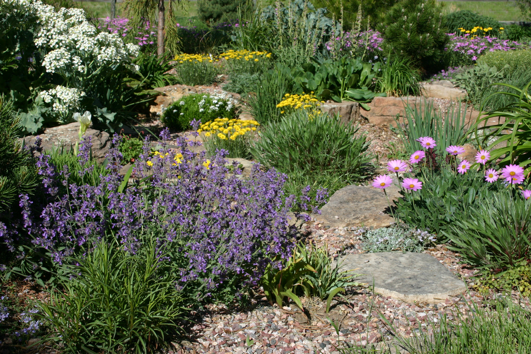
\includegraphics[width=.8\textwidth]{images/Austin-Y.png}
    \caption{Representation of Xeriscaping}
    \label{fig:AustinY}
\end{figure}
\subsubsection{Landscaping Design Decision Matrix}
Alternatives 1 to 3 were evaluated based on five categories: cost, overall lifetime durability, general aesthetics, environmental benefit, and time required for placement. Each category for each 	alternative was given a score between 1 and 10, with 10 as the most favorable and 1 as the least favorable. 

%IGNORE ME - Dane will handle this!
\begin{table}[H]
\centering
\caption{Landscaping Design Decision Matrix}
\label{my-label}
\resizebox{\textwidth}{!} & \textbf{20\%} & \textbf{20\%} & \textbf{20\%} & \textbf{20\%} & \textbf{100\%} \\
\rowcolor[HTML]{DAE8FC} 
\textbf{Option} & \textbf{Cost} & \textbf{Durability} & \textbf{Aesthetics} & \textbf{Environmental Benefit} & \textbf{Placement} & \textbf{Score} \\
\rowcolor[HTML]{9AFF99} 
\textbf{Tall Fescue} & 9 & 9 & 10 & 7 & 10 & 90 \\
\textbf{Xeriscaping} & 6 & 10 & 8 & 10 & 5 & 78 \\
\end{tabular}%
}
\end{table}
%IGNORE ME - Dane will handle this!

\subsubsection{Landscaping Design Conclusions and Recommendations}
Based on the design matrix tall fescue scored the highest at 90 percent and xeriscaping coming in at 78 percent. This is mostly due to the work needed at the beginning to design and place xeriscaping local plants as well as the overall cost difference. Tall fescue also is easy to place as well as easy to maintain requiring minimal irrigation as well as labor. While xeriscaping is the much bettter choice in order to save water it is a design that works best in areas of dry climate and desert areas. The project is located in a flood plain area and will potentially require minimal stored water irrigation anyway due to weather conditions for the area. Therefore tall fescue is the chosen alternative for the landscaping portion of the project.
\newpage
\subsection{Foundations}
For the landscaping portion of the new proposed Shelby County Combined Cycle Power Plant two alternatives were considered for recommendation to the client Kiewit Power. The alternatives were considered based upon cost, overall strength, durability, material use, and potential settlement.

\subsubsection{Alternative 1 - Spread Footing}
Spread footing foundations are the most common type of foundation particular in the residential sector. These typical foundations lay on top of the soil and are considered a shallow foundation. They do require reinforcement in most situations and are good in areas where settlement and swell of the soil underneath the footing is not a major issue. Shallow foundations typically use less material making it much more cost effective having generally the same thickness throughout the process. Thus making it easier to construct but also allowing a higher risk of cracks along with settlement in the foundation. An example is shown below in \textbf{figure \ref{fig:Austin1}}

	\textbf{Advantages:}
\begin{itemize}
\item  Easily/quickly constructed
\item  Affordable cost
\item  Minimal material use
\end{itemize}
   
   	\textbf{Disadvantages:}
\begin{itemize}
\item  High risk of cracking/settlement
\item  Subject to torsion, uplift, compressive, lateral, and moment loading
\item  Minimal durability over lifespan 
\item  Minimal protection against liquefaction
\item  Minimal seismic protection
\end{itemize}


\begin{figure}[H]
    \centering
    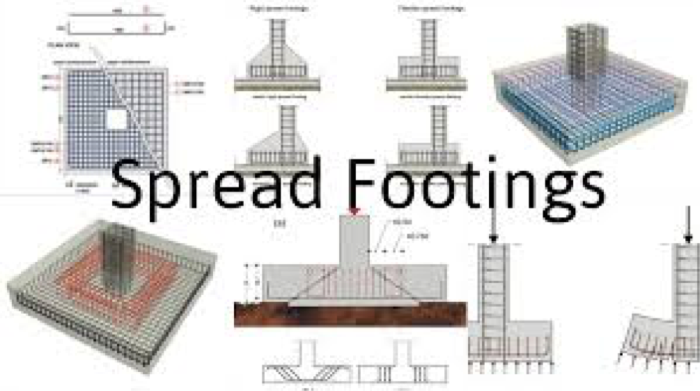
\includegraphics[width=.5\textwidth]{images/Austin1.png}
    \caption{Representation of Spread Footing}
    \label{fig:Austin1}
\end{figure}

\subsubsection{Alternative 2 - Deep Foundation}
Deep foundations are designed mostly for heavier structures and based on the fact that the load-carrying capacity of soils generally increases with depth, and deep foundations engage a larger volume of soil. These type of foundations are generally used in areas where the soils are poor and usually transfer loads through weak, compressible soils to underlying competent soils or rock. The method being considered for the project is the process of driven steel piles which is the most common form used and are typical driven but can end up needing bored holes in order to be driven properly increasing labor and overall cost. This type of foundation helps increase strength against static as well as seismic loads allowing the foundation to be connected to the driven pile. The typical cost is more expensive for this general type due to equipment requirements as well as overall material cost due to steel cost. An example is shown in \textbf{figure \ref{fig:Austin2}}

	\textbf{Advantages:}
\begin{itemize}
\item  Few material requirements
\item  Resist cracking/settlement
\item  Resist torsion, uplift, compressive, lateral, and moment loading
\item  Increases strength for static as well as seismic loads
\item  Provides earth retention
\item  High durability over lifespan
\end{itemize}
        
	\textbf{Disadvantages:}
\begin{itemize}
\item  Steeper cost
\item  Minimal mitigation against liquefaction
\item  Not recommended for soils with poor drainage quality
\item  Possibility of heaving of soil during driving process
\item  Potentially more heavy equipment and labor cost
\end{itemize}

\begin{figure}[H]
    \centering
    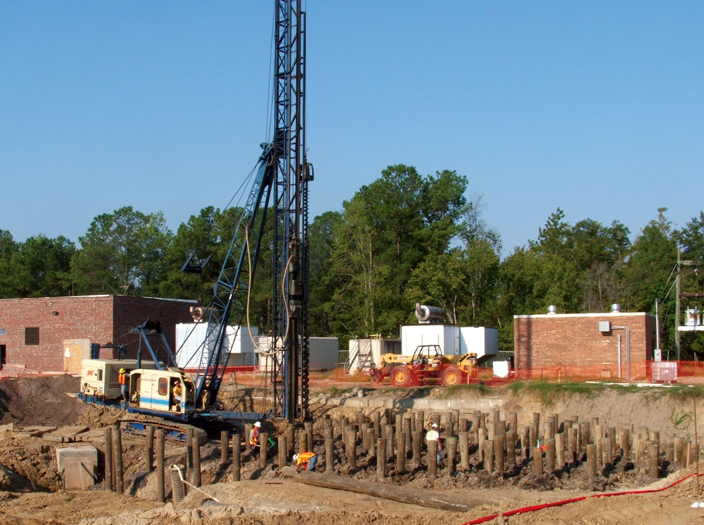
\includegraphics[width=.4\textwidth]{images/Austin2.png}
    \caption{Representation of Deep Foundation}
    \label{fig:Austin2}
\end{figure}
 
\subsubsection{Alternative 3 - Vibro Replacement}
Vibro replacement is the construction of dense aggregate columns or stone columns with a down-hole vibrator suspended from a crane or specially built rig. This process densifies and and reinforces all soils. The process involves penetrating the soil to the required depth then using a wet top-feed process in which crushed stone or concrete can be fed through while vibration occurs. Once the lift is finished then the rig pull up the rig and sets it back down allowing for compaction within the soil and then repeats the process until the material used reaches the top of the soil. This is a little more of a complex process and requires the proper equipment. The overall cost is still very economical while also reducing more of the issues accompanying foundation design. An example is shown in \textbf{figure \ref{fig:Austin3}}

	\textbf{Advantages:}
\begin{itemize}
\item  Affordable cost
\item Increase bearing capacity
\item  Decrease settlement
\item  Mitigate liquefaction
\item  Cheaper than driven piles
\item  High durability over lifespan
\item  Few/reusable material requirements
\item  Resist cracking/settlement
\item  Resist torsion, uplift, compressive, lateral, and moment loading
\item  Increases strength for static as well as seismic loads
\item  Provides earth retention
\end{itemize}
        
	\textbf{Disadvantages:}
\begin{itemize}
\item Vibro replacement is only effective on granular and non-cohesive soils.
\item Not suitable for sites with contaminated land for vibratory techniques that use water jetting.
\end{itemize}
    
\begin{figure}[H]
    \centering
    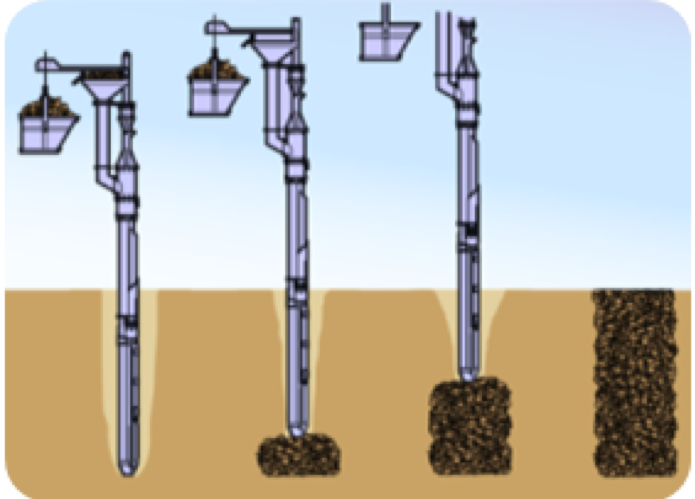
\includegraphics[width=.35\textwidth]{images/Austin3.png}
    \caption{Representation of Vibro Replacement}
    \label{fig:Austin3}
\end{figure}    
    
\subsubsection{Foundation Design Decision Matrix}
Alternatives 1 to 3 were evaluated based on five categories: based upon cost, overall strength, durability, material use, and potential against settlement. Each category for each 	alternative was given a score between 1 and 10, with 10 as the most favorable and 1 as the least favorable. 
    
	\begin{table}[H]
	\centering
	\caption{Foundation Design Decision Matrix}
\label{my-label}
	\resizebox{\textwidth}{!} & \textbf{20\%} & \textbf{20\%} & \textbf{20\%} & \textbf{20\%} & \textbf{100\%} \\
	\rowcolor[HTML]{DAE8FC} 
	\textbf{Option} & \textbf{Cost} & \textbf{Strength} & \textbf{Durability} & \textbf{Material Use} & \textbf{Settlement} & \textbf{Score} \\
	\textbf{Spread Footing} & 9 & 2 & 2 & 9 & 3 & 50 \\
\textbf{Deep Foundation} & 5 & 8 & 8 & 6 & 9 & 72 \\
\rowcolor[HTML]{9AFF99} 
	\textbf{Vibro Replacement} & 8 & 10 & 10 & 8 & 10 & 92 \\
	\end{tabular}%
	}
	\end{table}
    
\subsubsection{Foundation Design Conclusions and Recommendations}
As shown in the decision matrix vibro replacement received the highest score of 92 percent with deep foundation being the second highest score. TechnologyBin believes the other alternatives are good options for the project but based on the requirements lain out by Keiwit and overall plant design vibro replacement meets the most requirements while also being the most cost effective option. It is also environmentally friendly with the practical use of crushed stone or concrete which TechnologyBin utilizes daily. TechnologyBin has also had extensive experience with this process in the past. 
\newpage
\subsection{Drainage Routing}
Optional Text Here:

\subsubsection{Alternative 1 - Name of Alternative}
Text Here:

\subsubsection{Alternative 2 - Name of Alternative}
Text Here:

\subsubsection{Drainage Design Decision Matrix}
Text Here:

%IGNORE ME - Dane will edit this!
\begin{table}[H]
\centering
\caption{Drainage Design Decision Matrix}
\label{my-label}
\resizebox{\textwidth}{!} & \textbf{20\%} & \textbf{20\%} & \textbf{20\%} & \textbf{20\%} & \textbf{100\%} \\
\rowcolor[HTML]{DAE8FC} 
\textbf{Option} & \textbf{Attribute 1} & \textbf{Attribute 2} & \textbf{Attribute 3} & \textbf{Attribute 4} & \textbf{Attribute 5} & \textbf{Score} \\
\textbf{Option A} & 0 & 0 & 0 & 0 & 0 & 0 \\
\textbf{Option B} & 0 & 0 & 0 & 0 & 0 & 0 \\
\rowcolor[HTML]{9AFF99} 
\textbf{Option C} & 1 & 1 & 1 & 1 & 1 & 1 \\
\textbf{Option D} & 0 & 0 & 0 & 0 & 0 & 0
\end{tabular}%
}
\end{table}
%IGNORE ME - Dane will edit this!

\subsubsection{Drainage Design Conclusions and Recommendations}
Text Here:
\newpage
\subsection{Industrial Waste Water Treatment}
Optional Text Here:

\subsubsection{Alternative 1 - Name of Alternative}
Text Here:

\subsubsection{Alternative 2 - Name of Alternative}
Text Here:

\subsubsection{Waste Water Treatment Design Decision Matrix}
Text Here:

%IGNORE ME - Dane will edit this!
\begin{table}[H]
\centering
\caption{Waste Water Treatment Design Decision Matrix}
\label{my-label}
\resizebox{\textwidth}{!} & \textbf{20\%} & \textbf{20\%} & \textbf{20\%} & \textbf{20\%} & \textbf{100\%} \\
\rowcolor[HTML]{DAE8FC} 
\textbf{Option} & \textbf{Attribute 1} & \textbf{Attribute 2} & \textbf{Attribute 3} & \textbf{Attribute 4} & \textbf{Attribute 5} & \textbf{Score} \\
\textbf{Option A} & 0 & 0 & 0 & 0 & 0 & 0 \\
\textbf{Option B} & 0 & 0 & 0 & 0 & 0 & 0 \\
\rowcolor[HTML]{9AFF99} 
\textbf{Option C} & 1 & 1 & 1 & 1 & 1 & 1 \\
\textbf{Option D} & 0 & 0 & 0 & 0 & 0 & 0
\end{tabular}%
}
\end{table}
%IGNORE ME - Dane will edit this!

\subsubsection{Waste Water Treatment Conclusions and Recommendations}
Text Here:
\newpage
\subsection{Structural Design}
Concerning the structural design of the administrative building, three alternatives were evaluated. Each of these three alternative methods are suitable for supporting the loads present in this building and are commonly used in buildings of this size. The methods were evaluated using several relevant criteria including: cost, construction time, durability, and maintenance. 

\subsubsection{Alternative 1 - Structural Steel}
Structural steel is a very effective material when used to support building loads. This material offers many advantages in the construction phase of the project. Steel beams are a commonly used material that is readily available, and the members can be fabricated off-site and shipped to the construction site to be erected. This prevents the construction site from being cluttered with excess activity. This alternative also allows for very quick construction and versatile exterior facades such as glass curtain walls or non-structural bricks.

	\textbf{Advantages:}
\begin{itemize}
\item  Quick Construction
\item Versatile Exterior Design
\item Off-site Fabrication
\end{itemize}

	\textbf{Disadvantages:}
\begin{itemize}
\item High Fabrication Costs
\item Requires Extra Fireproofing
\end{itemize}

\begin{figure}[H]
    \centering
    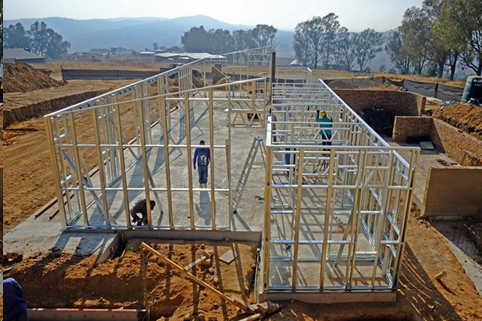
\includegraphics[width=.5\textwidth]{images/Structural1.png}
    \caption{Single Story Light Structural Steel Frame Construction}
    \label{fig:S_SSLSS}
\end{figure}

\subsubsection{Alternative 2 - Concrete Masonry Units}
Constructing a building out of concrete blocks offers many benefits and advantages to the life of the structure. Concrete masonry unit (CMU) will be used to support the load of the building in both in interior and exterior walls. The roof structure will be built on joints that span the distances between interior and exterior walls. Including insulation in the CMU will provide excellent thermal resistance properties and this will cut energy costs. CMU also provides great fire resistance, so the building will be very safe without the need for extra fireproofing.

\textbf{Advantages:}
\begin{itemize}
\item  Durable Material
\item High Thermal Resistance
\item No Additional Fireproofing Required
\end{itemize}

\textbf{Disadvantages:}
\begin{itemize}
\item Lack of Versatility in Exterior Facade
\item Slower Construction Process
\end{itemize}

\begin{figure}[H]
    \centering
    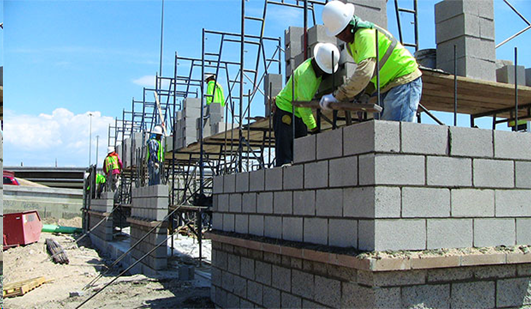
\includegraphics[width=.7\textwidth]{images/Structural2.png}
    \caption{Concrete Masonry Unit Construction}
    \label{fig:S_CMUC}
\end{figure}
\newpage
\subsubsection{Alternative 3 - Timber Framing}
Timber framing is an incredibly inexpensive and versatile load bearing method. Timber structures use renewable resources and allow for a fast construction process. With a concrete slab constructed underneath the structure, the walls are erected directly on the slab and timber joists in the roof structure span the spaces between load bearing walls. The versatility of timber construction allows for flexibility in the interior design of the space as well as the exterior facade.

\textbf{Advantages:}
\begin{itemize}
\item Inexpensive
\item Quick Construction
\item No Additional Fireproofing Required
\end{itemize}

\textbf{Disadvantages:}
\begin{itemize}
\item Lack of Versatility in Exterior Facade
\item Slower Construction Process
\end{itemize}


\begin{figure}[H]
    \centering
    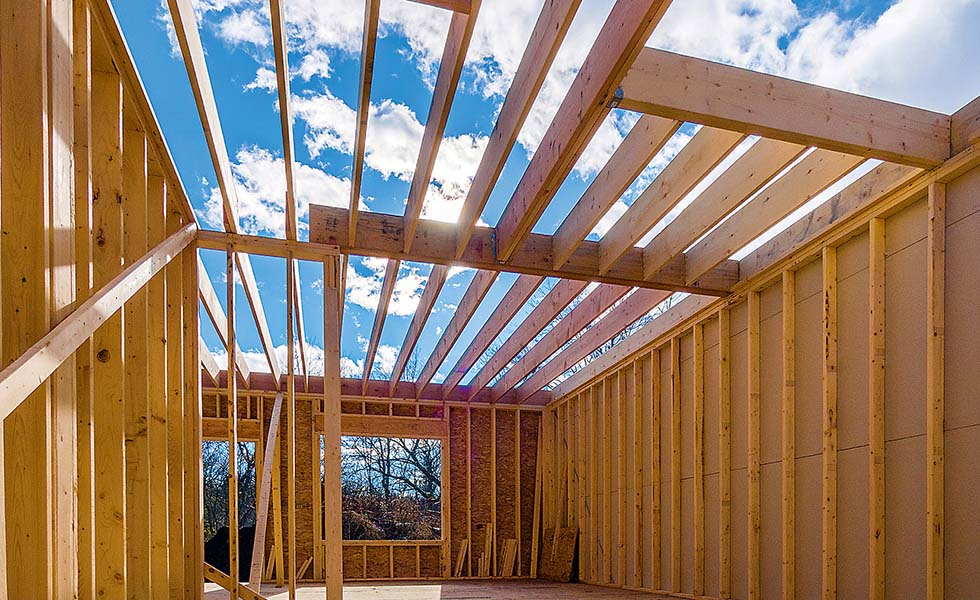
\includegraphics[width=.7\textwidth]{images/Structural3.png}
    \caption{Single Story Timber Construction}
    \label{fig:S_SSTC}
\end{figure}
\newpage
\subsubsection{Structural Design Decision Matrix}
Text Here:

%IGNORE ME - Dane will edit this!
\begin{table}[H]
\centering
\caption{Structural Design Decision Matrix}
\label{my-label}
\resizebox{\textwidth}{!} & \textbf{20\%} & \textbf{20\%} & \textbf{20\%} & \textbf{20\%} & \textbf{100\%} \\
\rowcolor[HTML]{DAE8FC} 
\textbf{Option} & \textbf{Attribute 1} & \textbf{Attribute 2} & \textbf{Attribute 3} & \textbf{Attribute 4} & \textbf{Attribute 5} & \textbf{Score} \\
\textbf{Option A} & 0 & 0 & 0 & 0 & 0 & 0 \\
\textbf{Option B} & 0 & 0 & 0 & 0 & 0 & 0 \\
\rowcolor[HTML]{9AFF99} 
\textbf{Option C} & 1 & 1 & 1 & 1 & 1 & 1 \\
\textbf{Option D} & 0 & 0 & 0 & 0 & 0 & 0
\end{tabular}%
}
\end{table}
%IGNORE ME - Dane will edit this!

\subsubsection{Structural Design Conclusions and Recommendations}
Text Here:
\newpage
\subsection{Pavement Materials}
O 

\subsubsection{Alternative 1 - Concrete}
Concrete is a very versatile material that bears large loads extremely well. For this reason, concrete would be a suitable material for parking lots and other roadways that expect to frequently see large loads. The maintenance costs are fairly low, because concrete does not develop holes or ruts as quickly as other materials might. With these advantages, concrete has a fairly high initial cost and long curing periods before it can be used.
\textbf{Advantages:}
\begin{itemize}
    \item Durability
    \item Less Future Maintenance
    \item Better Performance in Hot Weather
\end{itemize}
\textbf{Disadvantages:}
\begin{itemize}
    \item Long Curing Period
    \item High Initial Cost
    \item Corrosion by Winter Salting
\end{itemize}

\begin{figure}[H]
    \centering
    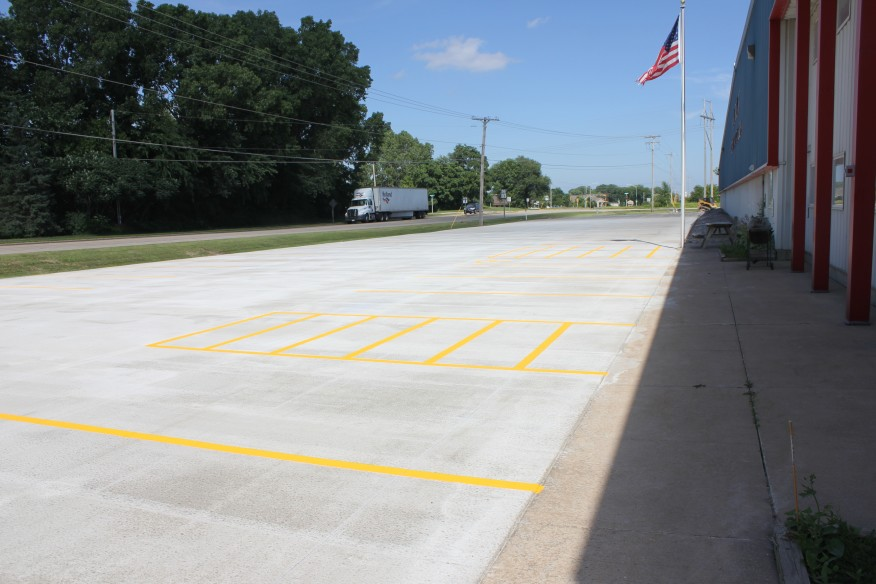
\includegraphics[width=.7\textwidth]{images/Pavement1.png}
    \caption{Concrete Pavement Parking lot}
    \label{fig:P_CPPL}
\end{figure}

\subsubsection{Alternative 2 - Asphalt}
Asphalt is a very common material for parking lots and other roadways because it offers many advantages. Asphalt can be installed and ready for traffic very quickly. With regular maintenance, asphalt can last up to 20 years before needing an overlay. Rutting and holes may form where frequent and heavy traffic loads are present. Asphalt also does not perform well in very hot conditions.
\textbf{Advantages:}
\begin{itemize}
    \item Fast Installation
    \item Low Initial Cost
    \item Effective Drainage
\end{itemize}
\textbf{Disadvantages:}
\begin{itemize}
    \item Requires Regular Maintenance
    \item Rutting and Holes Form Where Heavy Loads are Present
    \item Bad Performance in Hot Weather
\end{itemize}

\begin{figure}[H]
    \centering
    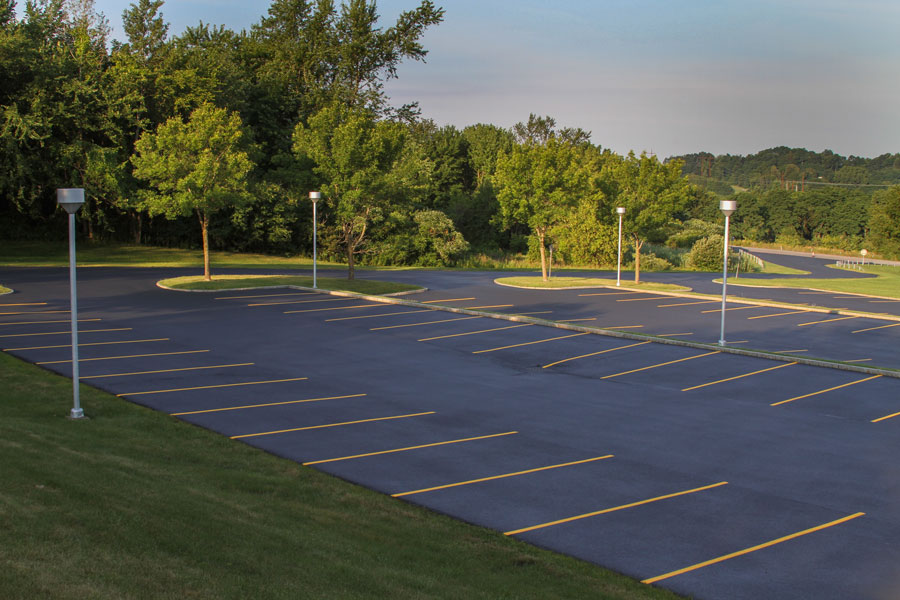
\includegraphics[width=.7\textwidth]{images/Pavement2.png}
    \caption{Asphalt Pavement Parking Lot}
    \label{fig:P_SAPPL}
\end{figure}

\subsubsection{Alternative 3 - Pervious Concrete}
Pervious Concrete is used less often than the previous two alternatives, but the material offers other benefits that make it suitable for a project this size. The benefits of pervious concrete include excellent drainage and less icing in winter conditions. In Figure 12, shown below, the area reserved for parked cars has significantly better drainage than the travel way. This material does take longer to install, and the initial cost is higher. 
\textbf{Advantages:}
\begin{itemize}
    \item Excellent Drainage
    \item Made from Recycled Materials
    \item Better Performance in Hot Weather
\end{itemize}
\textbf{Disadvantages:}
\begin{itemize}
    \item High Initial Cost
    \item Less Strength
    \item Requires Regular Maintenance to Clear Debris
\end{itemize}


\begin{figure}[H]
    \centering
    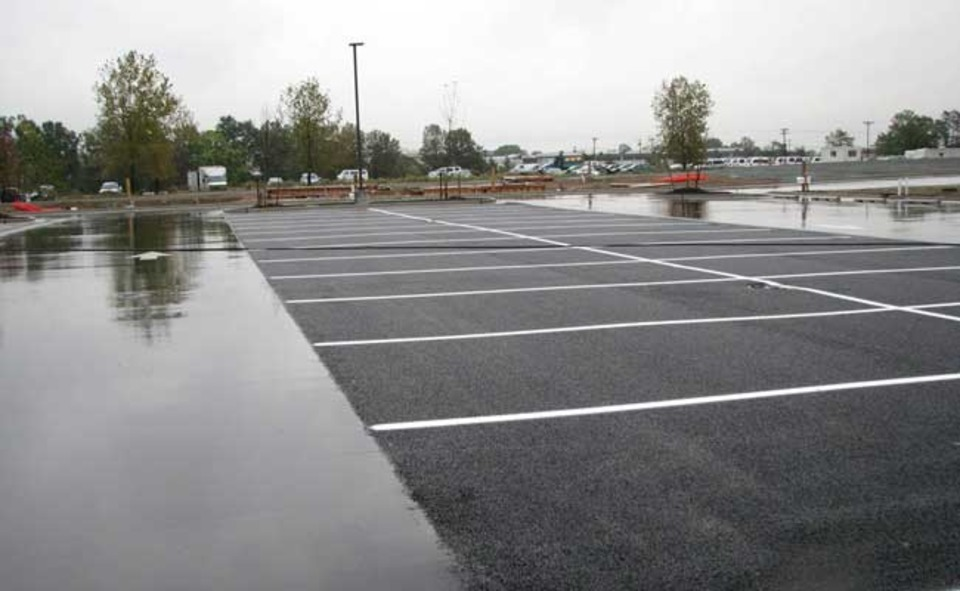
\includegraphics[width=.7\textwidth]{images/Pavement3.png}
    \caption{Pervious Concrete Pavement Parking Lot}
    \label{fig:P_PCPPL}
\end{figure}

\subsubsection{Pavement Materials Design Decision Matrix}
Text Here:

%IGNORE ME - Dane will edit this!
\begin{table}[H]
\centering
\caption{Pavement Materials Design Decision Matrix}
\label{my-label}
\resizebox{\textwidth}{!} & \textbf{20\%} & \textbf{20\%} & \textbf{20\%} & \textbf{20\%} & \textbf{100\%} \\
\rowcolor[HTML]{DAE8FC} 
\textbf{Option} & \textbf{Attribute 1} & \textbf{Attribute 2} & \textbf{Attribute 3} & \textbf{Attribute 4} & \textbf{Attribute 5} & \textbf{Score} \\
\textbf{Option A} & 0 & 0 & 0 & 0 & 0 & 0 \\
\textbf{Option B} & 0 & 0 & 0 & 0 & 0 & 0 \\
\rowcolor[HTML]{9AFF99} 
\textbf{Option C} & 1 & 1 & 1 & 1 & 1 & 1 \\
\textbf{Option D} & 0 & 0 & 0 & 0 & 0 & 0
\end{tabular}%
}
\end{table}
%IGNORE ME - Dane will edit this!

\subsubsection{Pavement Materials Design Conclusions and Recommendations}
Text Here:
\newpage 
\subsection{LEED Certification}
For LEED Certification several different alternatives were considered for recommendation to Kiewit. The alternatives were considered based on their contribution to Renewable Energy Production criteria regarding LEED Certification, their initial cost, tax credits, environmental impact, energy production, and required space.

\subsubsection{Alternative 1 - Photovoltaic Solar Panels}
Photovoltaic Panels are a common and reliable source of renewable energy that converts the sun’s Direct Current (DC) to an Alternating Current (AC). This can be used to provide energy to homes and businesses. For this alternative a 43-panel array was calculated to provide enough energy for LEED certification and was considered as an alternative energy source for the Administrative building. The panels could be fixed to the roof of the Administrative building or fixed above parking spaces to reduce the heat island effect and generate power unobstructed.


\textbf{Advantages:}
\begin{itemize}
\item Qualifies for up to three LEED credits
\item No carbon emissions
\item Return on investment (usually around 10 years)
\item Reduces overall electricity costs ( > 10\%)
\item Solar Tax Credit (30\%)
\item Can be integrated with Solar Thermal Arrays
\item Memphis, TN is in an optimal Latitude for solar energy
\end{itemize}
\textbf{Disadvantages:}
\begin{itemize}
\item High initial investment
\item Requires unobstructed space to produce electricity
\item Cannot produce electricity at night
\item Reduced energy production in cloudy weather or during winter months
\item Technology still in development
\end{itemize}

\begin{figure}[H]
    \centering
    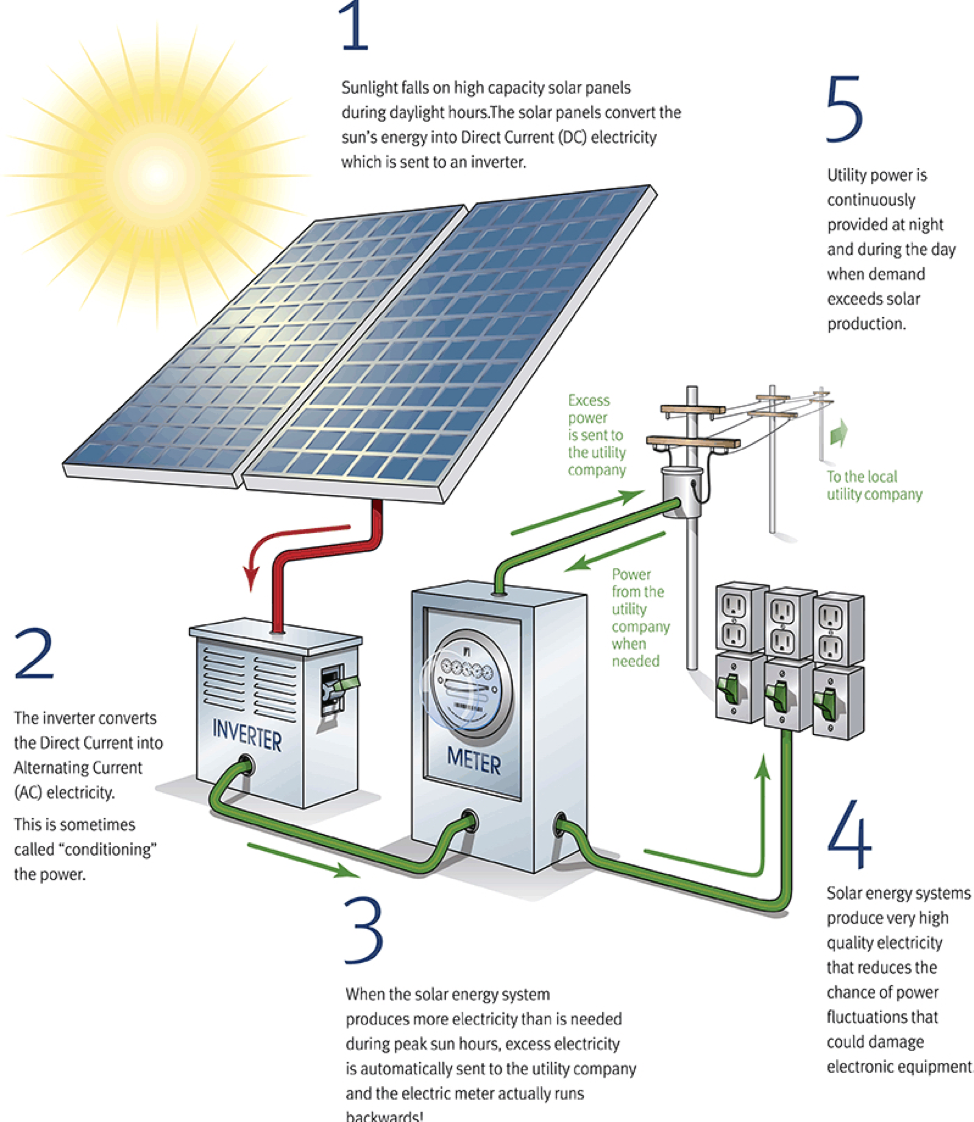
\includegraphics[width=.8\textwidth]{images/LEED1.png}
    \caption{Representation of a Photovoltaic Panel}
    \label{fig:PP_LEED}
\end{figure}
\newpage
\subsubsection{Alternative 2 - Solar Thermal}

Solar Thermal heating is a possible alternative to other electric or natural gas heating options for homes and businesses. While PV panels collect the Direct Current (DC), produced by sunlight, and convert it to Alternating Current (AC) to produce electricity, Solar Thermal arrays transfer the collected heat from the sun’s rays to a fluid and uses that stored, heated fluid to heat water, pipes, and other systems. Solar Thermal panels can easily be used and integrated with PV panels and can be fixed to the roof of the Administrative Building or fixed above parking spaces to reduce the heat island effect and generate power unobstructed.

Advantages:
\begin{itemize}
\item Qualifies for up to three LEED credits
\item No carbon emissions
\item Return on investment
\item Reduces electricity and natural gas costs
\item Solar Tax Credit (30\%)
\item Low maintenance costs
\item Can be integrated with PV arrays
\item Memphis, TN is in an optimal Latitude for solar energy
\end{itemize}
Disadvantages:
\begin{itemize}
\item High initial investment
\item Requires unobstructed space to produce collect heat
\item Cannot collect heat at night
\item Reduced heat collection in cloudy weather or during winter months
\item Technology still in development
\end{itemize}

\begin{figure}[H]
    \centering
    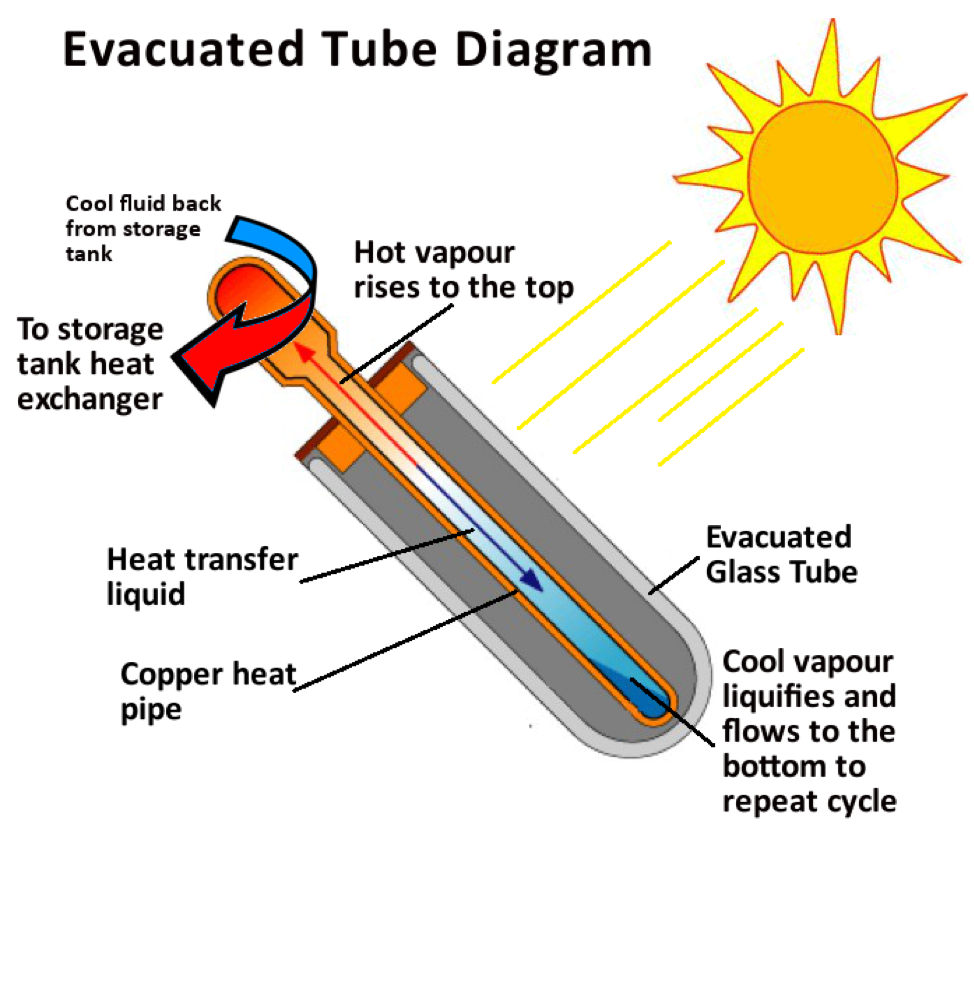
\includegraphics[width=.35\textwidth]{images/LEED2.png}
    \caption{Representation of Solar Thermal Heating unit}
    \label{fig:THU_LEED}
\end{figure}

\subsubsection{Alternative 3 - Wind}

Wind energy is a common and reliable energy source that uses the wind to spin a turbine to produce electricity. This can be used to produce energy for homes and businesses. For this alternative a 20kw turbine was calculated to provide enough energy for LEED certification and was considered as an alternative energy source for the Administrative building. A wind turbine can be installed on site, away from the Combined Cycle Power Plant.

Advantages:
\begin{itemize}
\item Qualifies for up to three LEED credits
\item No carbon emissions
\item Return on investment
\item Installation rebate / tax credit (50\%)
\item Operates day and night (90\% of the time)
\item Memphis, TN has optimal wind speeds for wind energy
\end{itemize}
Disadvantages:
\begin{itemize}
\item High initial investment
\item Requires substantial, unobstructed space to produce energy
\item Cannot produce energy if wind speeds are too high or too low
\item Reduce heat collection in cloudy weather or during winter months
\item Technology still in development
\item Can be considered unattractive
\item Potentially dangerous to avian species.
\end{itemize}

\newpage
\subsubsection{LEED Certification Design Decision Matrix}
Table \ref{table:LEEDMatrix} show the decision matrix used to assign weights to the categories used while determining possible LEED alternatives. The categories selected were initial cost, tax credits, environmental impact, energy produced, and required space. The categories were calculated to have scores between one and ten, with ten being a superior option and 1 being an inferior option. The categories were weighted based upon their impact on project cost, space, and future returns. Higher weights were placed on initial cost and energy produced annually due to the impact the options will have on project finances. Moderate weights were placed on tax credits and the required space each system requires due to possible return on investments and space limitations. Finally, a lower weight was placed on environmental impact due to all options having minimal negative effects on the environment. The scores were initially calculated with one being the superior score and ten being the inferior score, but were converted to the inverse for convenience on the client

%IGNORE ME - Dane will edit this!
\begin{table}[H]
\centering
\caption{LEED Certification Category Comparison}
\label{my-label}
\resizebox{\textwidth}{!} & \multicolumn{1}{l|}{\cellcolor[HTML]{ECF4FF}1} & \multicolumn{1}{l|}{\cellcolor[HTML]{ECF4FF}2} & \multicolumn{1}{l|}{\cellcolor[HTML]{ECF4FF}4,300 sf} \\ \cline{2-6} 
\rowcolor[HTML]{ECF4FF} 
\multicolumn{1}{l|}{\cellcolor[HTML]{DAE8FC}Solar Thermal} & \multicolumn{1}{l|}{\cellcolor[HTML]{ECF4FF}\$2,000} & \multicolumn{1}{l|}{\cellcolor[HTML]{ECF4FF}30\%} & \multicolumn{1}{l|}{\cellcolor[HTML]{ECF4FF}3} & \multicolumn{1}{l|}{\cellcolor[HTML]{ECF4FF}10} & \multicolumn{1}{l|}{\cellcolor[HTML]{ECF4FF}4,300 sf} \\ \cline{2-6} 
\rowcolor[HTML]{ECF4FF} 
\multicolumn{1}{l|}{\cellcolor[HTML]{DAE8FC}Wind Turbine} & \multicolumn{1}{l|}{\cellcolor[HTML]{ECF4FF}\$100,000} & \multicolumn{1}{l|}{\cellcolor[HTML]{ECF4FF}50\%} & \multicolumn{1}{l|}{\cellcolor[HTML]{ECF4FF}10} & \multicolumn{1}{l|}{\cellcolor[HTML]{ECF4FF}1} & \multicolumn{1}{l|}{\cellcolor[HTML]{ECF4FF}65,340 sf} \\ \cline{2-6} 
\end{tabular}%
}
\end{table}


\begin{table}[H]
\centering
\caption{LEED Certification Design Decision Matrix}
\label{table:LEEDMatrix}
\resizebox{\textwidth}{!}{%
\begin{tabular}{llllllll}
 & 0.25 & 0.2 & 0.1 & 0.25 & 0.2 &  &  \\
\rowcolor[HTML]{DAE8FC} 
\textbf{Option} & Initial Cost & Tax Credit & Environmental Impact & Energy Produced & Required Space & \textbf{Total} & \cellcolor[HTML]{9AFF99}\textbf{Score} \\ \cline{2-8} 
\rowcolor[HTML]{ECF4FF} 
\multicolumn{1}{l|}{\cellcolor[HTML]{DAE8FC}Photovoltaic Panels} & \multicolumn{1}{l|}{\cellcolor[HTML]{ECF4FF}2.5} & \multicolumn{1}{l|}{\cellcolor[HTML]{ECF4FF}1.4} & \multicolumn{1}{l|}{\cellcolor[HTML]{ECF4FF}0.1} & \multicolumn{1}{l|}{\cellcolor[HTML]{ECF4FF}0.5} & \multicolumn{1}{l|}{\cellcolor[HTML]{ECF4FF}0.2} & \multicolumn{1}{l|}{\cellcolor[HTML]{DAE8FC}4.7} & \multicolumn{1}{l|}{\cellcolor[HTML]{9AFF99}5.3} \\ \cline{2-8} 
\rowcolor[HTML]{ECF4FF} 
\multicolumn{1}{l|}{\cellcolor[HTML]{DAE8FC}Solar Thermal} & \multicolumn{1}{l|}{\cellcolor[HTML]{ECF4FF}0.3} & \multicolumn{1}{l|}{\cellcolor[HTML]{ECF4FF}1.4} & \multicolumn{1}{l|}{\cellcolor[HTML]{ECF4FF}0.3} & \multicolumn{1}{l|}{\cellcolor[HTML]{ECF4FF}2.5} & \multicolumn{1}{l|}{\cellcolor[HTML]{ECF4FF}0.2} & \multicolumn{1}{l|}{\cellcolor[HTML]{DAE8FC}4.7} & \multicolumn{1}{l|}{\cellcolor[HTML]{9AFF99}5.3} \\ \cline{2-8} 
\rowcolor[HTML]{ECF4FF} 
\multicolumn{1}{l|}{\cellcolor[HTML]{DAE8FC}Wind Turbine} & \multicolumn{1}{l|}{\cellcolor[HTML]{ECF4FF}2.4} & \multicolumn{1}{l|}{\cellcolor[HTML]{ECF4FF}1} & \multicolumn{1}{l|}{\cellcolor[HTML]{ECF4FF}1} & \multicolumn{1}{l|}{\cellcolor[HTML]{ECF4FF}0.3} & \multicolumn{1}{l|}{\cellcolor[HTML]{ECF4FF}2} & \multicolumn{1}{l|}{\cellcolor[HTML]{DAE8FC}6.7} & \multicolumn{1}{l|}{\cellcolor[HTML]{9AFF99}3.3} \\ \cline{2-8} 
\end{tabular}%
}
\end{table}
%IGNORE ME - Dane will edit this!
\newpage
\subsubsection{LEED Certification Design Conclusions and Recommendations}
TechnologyBin is recommending the client uses Photovoltaic Panels as an alternate energy source for the project. While Solar Thermal systems had the same score as Photovoltaic Panels, PV panels will produce more energy than a ST system while having return on investment in approximately the same time. However, ST systems have the lowest of initial costs by a large margin, can be easily integrated with PV arrays and both systems can be used in similar spaces. A Wind Turbine as an alternative is superior to both options for electricity generation, comparable to PV for initial costs, and has a higher tax credit than PV and ST but requires a large amount of space and must be certain distances away form other buildings and structures.


\subsection{Lighting Design}

TechnologyBin has developed three design alternatives regarding the lighting design for the combined cycle plan. While the Scope of Work provided by Kiewit designates LED lighting for all plant lighting, the following analysis on alternative serve to reiterate why LED lighting is the most sustainable and favorable method for lighting design. Considerations when comparing the lighting alternatives include:\\
\begin{itemize}
    \item Initial and operational costs
    \item Environmental Impact and LEED potential
    \item Light trespass and glare reduction
    \item Natural lighting integration and energy efficiency
    \item Light distribution and categories of lighting
    \newline
\end{itemize}
\newpage
\subsubsection{Alternative 1 - Incandescent Lighting}

Incandescent lighting works by incandescence and emits light by heating the filament. This type of bulb is widely used and has an extremely wide range of sizes, wattages, and voltages for different purposes. However, incandescent bulbs have the lowest efficiency and shortest lifespan when compared to fluorescent bulbs and LED lighting. In addition, incandescent bulbs have been slowly phased out of the market.\\
\newline
\textbf{Advantages:}
\begin{itemize}
    \item Extremely wide range
    \item Extremely wide range of styles and sizes
    \item Lower initial cost than alternatives
    \item No toxic materials
\end{itemize}
\textbf{Disadvantages:}
\begin{itemize}
    \item Low durability and short lifespan
    \item Very low energy efficiency
    \item Moderately sensitive to low temperatures and humidity
    \item High level of carbon dioxide emissions
\end{itemize}

\subsubsection{Alternative 2 - Fluorescent Lighting}

Fluorescent and compact fluorescent lighting operates using the low-pressure gas discharge principle and use fluorescence to produce light. This type of lighting can be used for a variety of applications due having a wide range of colors. Fluorescent lighting is more efficient than incandescent lighting, but experiences more issues with durability than LED lighting.\\

\newline
\textbf{Advantages}
\begin{itemize}
    \item Wide range of styles and sizes
    \item Lifespan is over six times the length of incandescent bulbs
\end{itemize}
\textbf{Disadvantages:}
\begin{itemize}
    \item Low durability
    \item Requires time to turn on
    \item Sensitive to humidity and extreme temperatures
    \item Contains mercury
\end{itemize}

\subsubsection{Alternative 3 - Light-Emitting Diode (LED) Lighting}

A light-emitting diode light bulb is a type of solid-state lighting that uses a semiconductor to emit light when current flows through it. LEDs are a sustainable lighting alternative to both incandescent bulbs and fluorescent bulbs. While LEDs have a higher initial cost, they have a much longer lifespan and higher efficiency than other lighting sources.\\




\subsubsection{Lighting Design Decision Matrix}
Alternatives 1 to 3 were evaluated based on six categories: initial cost, annual operating cost, life span, CO2 emissions, heat emitted, and LEED potential. Each category for each alternative was given a score between 1 and 10, with 10 as the most favorable and 1 as the least favorable. Each category was then assigned a weight that represents their importance with respect to Kiewit’s requirements and to the scope of lighting design. These weights were used to calculate final scores for LED lighting, fluorescent lighting, and incandescent lighting to determine the most suitable alternative. The most favorable alternative of these three was LED lighting with a score of 9.61 out of 10.

%IGNORE ME - Dane will edit this!
\begin{table}[H]
\centering
\caption{Lighting Category Comparison}
\label{my-label}
\resizebox{\textwidth}{!}{%
\begin{tabular}{lllllll}
\rowcolor[HTML]{DAE8FC} 
\textbf{Option} & Initial Cost & Annual Operating Cost & Life Span (hours) & CO2 Emissions & Heat Emitted & LEED Potential \\ \cline{2-7} 
\rowcolor[HTML]{ECF4FF} 
\multicolumn{1}{l|}{\cellcolor[HTML]{DAE8FC}LED} & \multicolumn{1}{l|}{\cellcolor[HTML]{ECF4FF}High} & \multicolumn{1}{l|}{\cellcolor[HTML]{ECF4FF}\$32.85/year} & \multicolumn{1}{l|}{\cellcolor[HTML]{ECF4FF}50,000} & \multicolumn{1}{l|}{\cellcolor[HTML]{ECF4FF}451 lb/year} & \multicolumn{1}{l|}{\cellcolor[HTML]{ECF4FF}3.4 Btu/hr} & \multicolumn{1}{l|}{\cellcolor[HTML]{ECF4FF}High} \\ \cline{2-7} 
\rowcolor[HTML]{ECF4FF} 
\multicolumn{1}{l|}{\cellcolor[HTML]{DAE8FC}Fluorescent} & \multicolumn{1}{l|}{\cellcolor[HTML]{ECF4FF}Moderate} & \multicolumn{1}{l|}{\cellcolor[HTML]{ECF4FF}\$76.65/year} & \multicolumn{1}{l|}{\cellcolor[HTML]{ECF4FF}8,000} & \multicolumn{1}{l|}{\cellcolor[HTML]{ECF4FF}1051 lb/year} & \multicolumn{1}{l|}{\cellcolor[HTML]{ECF4FF}30 Btu/hr} & \multicolumn{1}{l|}{\cellcolor[HTML]{ECF4FF}Moderate} \\ \cline{2-7} 
\rowcolor[HTML]{ECF4FF} 
\multicolumn{1}{l|}{\cellcolor[HTML]{DAE8FC}Incandescent} & \multicolumn{1}{l|}{\cellcolor[HTML]{ECF4FF}Low} & \multicolumn{1}{l|}{\cellcolor[HTML]{ECF4FF}\$329.59/year} & \multicolumn{1}{l|}{\cellcolor[HTML]{ECF4FF}1,200} & \multicolumn{1}{l|}{\cellcolor[HTML]{ECF4FF}4500 lb/year} & \multicolumn{1}{l|}{\cellcolor[HTML]{ECF4FF}85 Btu/hr} & \multicolumn{1}{l|}{\cellcolor[HTML]{ECF4FF}Low} \\ \cline{2-7} 
\end{tabular}%
}
\end{table}


\begin{table}[H]
\centering
\caption{Lighting Design Decision Matrix}
\label{my-label}
\resizebox{\textwidth}{!}{%
\begin{tabular}{llllllll}
 & 0.2 & 0.25 & 0.25 & 0.10 & 0.10 & 0.1 &  \\
\rowcolor[HTML]{DAE8FC} 
\textbf{Option} & Initial Cost & Annual Operating Cost & Life Span & CO2 Emission & Heat Emitted & LEED Potential & \cellcolor[HTML]{9AFF99}\textbf{Score} \\ \cline{2-8} 
\rowcolor[HTML]{ECF4FF} 
\multicolumn{1}{l|}{\cellcolor[HTML]{DAE8FC}LED} & \multicolumn{1}{l|}{\cellcolor[HTML]{ECF4FF}2} & \multicolumn{1}{l|}{\cellcolor[HTML]{ECF4FF}2.25} & \multicolumn{1}{l|}{\cellcolor[HTML]{ECF4FF}2.5} & \multicolumn{1}{l|}{\cellcolor[HTML]{ECF4FF}0.9} & \multicolumn{1}{l|}{\cellcolor[HTML]{ECF4FF}0.96} & \multicolumn{1}{l|}{\cellcolor[HTML]{ECF4FF}1} & \multicolumn{1}{l|}{\cellcolor[HTML]{9AFF99}9.61} \\ \cline{2-8} 
\rowcolor[HTML]{ECF4FF} 
\multicolumn{1}{l|}{\cellcolor[HTML]{DAE8FC}Fluorescent} & \multicolumn{1}{l|}{\cellcolor[HTML]{ECF4FF}1} & \multicolumn{1}{l|}{\cellcolor[HTML]{ECF4FF}1.92} & \multicolumn{1}{l|}{\cellcolor[HTML]{ECF4FF}0.5} & \multicolumn{1}{l|}{\cellcolor[HTML]{ECF4FF}0.77} & \multicolumn{1}{l|}{\cellcolor[HTML]{ECF4FF}0.65} & \multicolumn{1}{l|}{\cellcolor[HTML]{ECF4FF}0.5} & \multicolumn{1}{l|}{\cellcolor[HTML]{9AFF99}5.33} \\ \cline{2-8} 
\rowcolor[HTML]{ECF4FF} 
\multicolumn{1}{l|}{\cellcolor[HTML]{DAE8FC}Incandescent} & \multicolumn{1}{l|}{\cellcolor[HTML]{ECF4FF}0.2} & \multicolumn{1}{l|}{\cellcolor[HTML]{ECF4FF}0.25} & \multicolumn{1}{l|}{\cellcolor[HTML]{ECF4FF}0.25} & \multicolumn{1}{l|}{\cellcolor[HTML]{ECF4FF}0.1} & \multicolumn{1}{l|}{\cellcolor[HTML]{ECF4FF}0.1} & \multicolumn{1}{l|}{\cellcolor[HTML]{ECF4FF}0.1} & \multicolumn{1}{l|}{\cellcolor[HTML]{9AFF99}1} \\ \cline{2-8} 
\end{tabular}%
}
\end{table}
%IGNORE ME - Dane will edit this!
\newpage
\subsubsection{Lighting Design Conclusion and Recommendations}
As seen in \textbf{figure \ref{L_L1}}, while incandescent lighting has a lower initial cost, the cost per hour of illumination for incandescent bulbs increases at a much greater rate than the rates of both compact fluorescent bulbs (CFLs) and LED bulbs. Meanwhile, both CFL lighting and LED lighting maintain much lower costs per day. 

\begin{figure}[H]
    \centering
    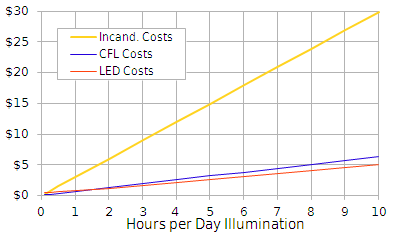
\includegraphics[width=.8\textwidth]{images/Lighting1.png}
    \caption{Average yearly costs for all bulbs}
    \label{L_L1}
 \end{figure}
\newpage 
\textbf{Figure \ref{L_L4}} shows the amount of electricity used by four different bulb types: incandescent, halogen, CFL, and LED. As seen below, incandescent lighting requires much more energy to operate than CFLs and LEDs at the same light output. In addition, while CFLs and LEDs both have low electricity use per amount of luminous flux, LEDs still use less energy than CFLs.

\begin{figure}[H]
    \centering
    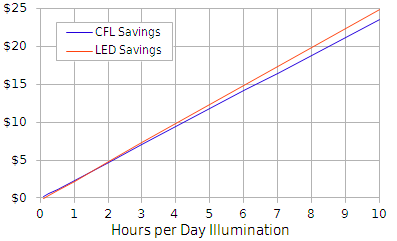
\includegraphics[width=.8\textwidth]{images/Lighting2.png}
    \caption{Average yearly savings for CFL and LED}
    \label{L_L3}
 \end{figure}
 \newpage


\begin{figure}[H]
    \centering
    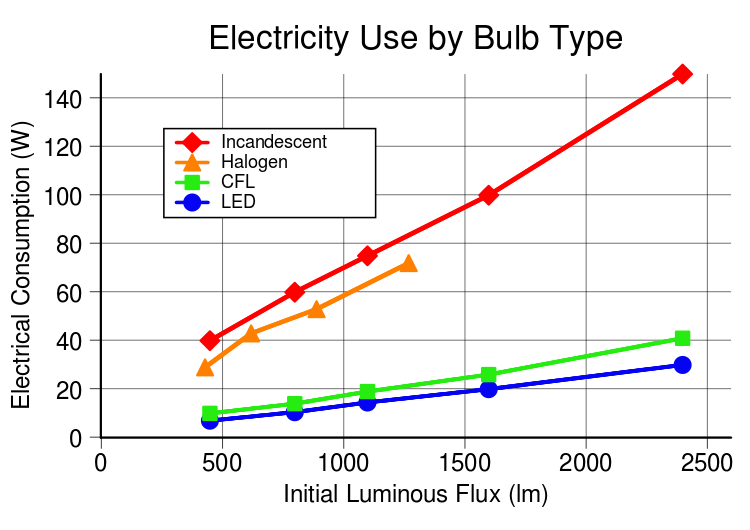
\includegraphics[width=.8\textwidth]{images/Lighting3.png}
    \caption{Electricity Use by Bulb Type}
    \label{L_L4}
 \end{figure}
 
TechnologyBin recommends the use of LED lighting over fluorescent and incandescent lighting because LEDs have an exceptionally higher life span and are more sustainable and efficient. Incorporating natural lighting is also recommended for LEED and sustainability reasons – using natural lighting in addition to LED lighting is more sustainable and can lower operational costs because less energy is needed for lighting during the day. Daylighting has also been shown to improve employee productivity and efficiency. However, incorporating natural lighting may increase structural costs and require a temperature regulation system.
\newpage
\section{Conclusion}
TechnologyBin has provided alternatives analyses covering landscaping, drainage routing, structural design, pavement materials, LEED certification, and lighting design for the combined cycle power plant. Each category was evaluated on design criteria such as sustainability, cost, life span and durability, and environmental impact. These values were then weighted to determine a common scale by which to compare alternatives. The recommendations made for each category are detailed below.

\subsection{Landscaping}
The alternatives considered for landscaping were....
The alternative x was chosen because....

\subsection{Drainage Routing}
The alternatives considered for drainage routing were....
The alternative x was chosen because....

\subsection{Structural Design}
The alternatives considered for structural design were....
The alternative x was chosen because....

\subsection{Pavement Materials}
The alternatives considered for pavement material were....
The alternative x was chosen because....

\subsection{LEED Certification}
For LEED certification, TechnologyBin evaluated three types of sustainable energy sources: photovoltaic solar panels, solar thermal heating, and wind turbines. These alternatives were compared in the categories of initial cost, tax credit, environmental impact, energy produced and required space. TechnologyBin recommends that Kiewit use photovoltaic panels as an alternative energy source for the combined cycle plant, as PV panels will produce more energy than a solar thermal system and requires much less space than wind turbines.

\subsection{Lighting Design}
Three alternatives were evaluated for lighting design: incandescent lighting, fluorescent lighting, and LED lighting. TehcnologyBin recommends LED lighting for its higher energy efficiency, much longer life span, and lower costs. In addition, LED lighting is much more sustainable than both alternatives, which helps meet the project's LEED goals. Incorporation of natural lighting is also recommended to promote sustainability and to lower lighting costs further.

\section{Appendices}
\end{document}
